\documentclass[11pt]{article}

% Change "review" to "final" to generate the camera-ready version.
\usepackage[review]{acl}

% Standard package includes
\usepackage{times}
\usepackage{latexsym}
\usepackage[T1]{fontenc}
\usepackage[utf8]{inputenc}
\usepackage{microtype}
\usepackage{inconsolata}
\usepackage{graphicx}

% Math, tables
\usepackage{amsmath,amssymb}
\usepackage{booktabs}
\usepackage{multirow}
\usepackage{xcolor}
\usepackage{url}

\title{Reward-Channel Separability in Multimodal Chart RLVR:\\
A Cross-Rollout Bonus and a Negative-Sample Caveat}

\author{Anonymous ACL submission}

\begin{document}
\maketitle

\begin{abstract}
Recent chart-reasoning vision-language models are trained via
reinforcement learning with verifiable rewards (RLVR), typically
following the Chart-RVR pipeline \citep{chartrvr2025}: GRPO with
multi-component rewards covering format adherence, chart-type
identification, table reconstruction, and answer accuracy. GRPO's
symmetric advantage rule reinforces correct rollouts uniformly,
which can erode the reasoning diversity that supports coverage at
higher inference compute. We propose \textbf{HCPC}, a cross-rollout
bonus that aims to preserve diverse reasoning paths by conditioning
on ground-truth correctness and rewarding consistent extraction
together with diverse reasoning. On Qwen2.5-VL-3B, HCPC matches
GRPO on Pass@1 ($0.622$ vs.\ $0.630$) while producing more robust
correct-path behavior: $40.8\%$ of ChartQA test samples have all $4$
rollouts correct (vs.\ $38.6\%$), Pass@4 is highest at $0.828$
(vs.\ $0.816$), and table-dependence is stronger
($\Delta_{\text{tbl}}{=}{+}0.264$ vs.\ ${+}0.178$). As a comparison
point we also port Negative-Sample Reinforcement (NSR;
\citealp{zhu2025nsr}), a recent advantage rule from text-only math
RLVR that masks the gradient of correct rollouts to preserve
diversity. NSR ported unchanged collapses format compliance in chart
RLVR ($96.8\%\!\to\!31.6\%$ on ChartQA,
$98.8\%\!\to\!16.2\%$ on OOD ChartFC) and significantly hurts OOD
Pass@4 ($-3.8$\,pp, $p{=}0.028$); per-tag analysis localizes the
collapse to the structural tags the base model does not emit
unprompted. Adding HCPC to NSR improves over plain NSR on
\emph{every} ChartFC metric and matches GRPO on Pass@1
($0.632$ vs.\ $0.638$)---at near-zero format compliance
($17.8\%$ vs.\ $98.8\%$). The dissociation between recovered accuracy
and unrecovered format is evidence that the two travel through
separable reward channels in chart RLVR.
\end{abstract}

\section{Introduction}
\label{sec:intro}

Recent chart-reasoning vision-language models are trained with RLVR
\citep{chartrvr2025,chartr12025,bigcharts2025,distill-vcr-2025},
typically following the Chart-RVR recipe: GRPO \citep{deepseekmath}
with verifiable rewards for chart-type identification, table
reconstruction, process conformity, and answer accuracy. GRPO's
symmetric advantage rule reinforces correct rollouts uniformly. This
can be effective for in-distribution single-shot accuracy but tends
to over-commit the policy to one solution path, eroding the reasoning
diversity that supports coverage at higher $K$ in Pass@$K$ and that
helps under distribution shift \citep{chartrvr2025,zhu2025nsr}.

We propose Hierarchical Correct-Path Consistency
(\textbf{HCPC}), a cross-rollout bonus that aims to preserve diverse
reasoning paths in a structured way. HCPC conditions on ground-truth
correctness and, among the rollouts in a group that get the table and
answer right, rewards \emph{consistent} table extraction together
with \emph{diverse} reasoning traces. The level-specific
objective reflects the structure of chart reasoning---perception
admits one right answer while reasoning over the extracted table
admits many---and the GT-anchored filter ensures the bonus rewards
correct-path \emph{quality} rather than agreement among arbitrary
rollouts.

As a comparison point we port Negative-Sample Reinforcement
\citep[NSR;][]{zhu2025nsr}, a recent advantage rule from text-only
math RLVR that targets the same diversity-preservation goal by a
different route: masking the gradient of correct rollouts and
penalizing only incorrect ones. \citet{zhu2025nsr} show that NSR
matches or beats GRPO at Pass@$K$ on math benchmarks while
preserving diversity; whether that property transfers to a
multi-component, multimodal reward landscape is one of the questions
we test, and as we show in \S\ref{sec:nsr_collapse} the answer is no.
NSR and HCPC therefore enter the paper as two \emph{attempts} at
preserving correct-path diversity---one by removing positive
reinforcement, the other by adding structured positive
reinforcement---only one of which delivers in our setting.

\paragraph{Contributions.}

\begin{enumerate}
    \item \textbf{HCPC as a diversity-preserving reward
    (\S\ref{sec:hcpc}, \S\ref{sec:hcpc_grpo}).} On Qwen2.5-VL-3B,
    HCPC on top of GRPO matches the Chart-RVR baseline on Pass@1
    ($0.622$ vs.\ $0.630$, ns) and produces more robust correct-path
    behavior: $40.8\%$ all-4-correct rate (vs.\ $38.6\%$), Pass@4
    $0.828$ (vs.\ $0.816$, highest of all configurations), and
    table-dependence $\Delta_{\text{tbl}}{=}{+}0.264$
    (vs.\ ${+}0.178$). Differences are within paired-bootstrap noise
    individually at $n{=}500$, but all in the direction the
    cross-rollout signal is designed to produce.
    \item \textbf{An NSR-on-VLM transferability finding
    (\S\ref{sec:nsr_collapse}).} Porting NSR unchanged from text-only
    math collapses format compliance in chart RLVR
    ($96.8\%{\to}31.6\%$ on ChartQA, $98.8\%{\to}16.2\%$ on ChartFC)
    and significantly hurts OOD Pass@4 on ChartFC
    ($-3.8$\,pp, $p{=}0.028$). The mechanism is mechanical:
    Chart-RVR's structural rewards saturate quickly, so well-formed
    rollouts cross NSR's correctness threshold regardless of whether
    their answer is right, and NSR masks the gradient that would
    teach structured output. Per-tag analysis localizes the collapse
    to exactly the tags the base model does not emit unprompted.
    \item \textbf{HCPC mitigates NSR's OOD damage; format and
    accuracy are empirically separable
    (\S\ref{sec:dissociation}).} Adding HCPC to NSR improves over
    plain NSR on \emph{every} ChartFC metric---Pass@1 $+4.2$\,pp,
    Pass@4 $+1.0$\,pp, $\Delta_{\text{tbl}}$ $+0.061$, format
    $+1.6$\,pp---and matches GRPO on Pass@1 ($0.632$ vs.\ $0.638$) at
    \emph{near-zero} format compliance ($17.8\%$ vs.\ $98.8\%$).
    What is surprising is not that the two metrics can move
    differently, but that NSR+HCPC reaches GRPO-level answer accuracy
    via a mechanism that provides \emph{no positive gradient on
    correct rollouts}---the very gradient that would be needed to
    restore format. The recovery instead operates through a baseline
    shift in the GRPO advantage computation: HCPC's bonus on correct
    rollouts raises the group mean, making wrong-rollout advantages
    more negative under NSR's mask.
\end{enumerate}

\section{Background}
\label{sec:background}

\paragraph{Chart-RVR backbone.} We build on the multi-reward GRPO
pipeline of \citet{chartrvr2025}, with verifiable components for
format adherence, length, answer accuracy, surrogate tasks (chart type
and table reconstruction), and process conformity. Two of these
components are structural and easy to satisfy once learned: a
partial-credit format reward $R_{\text{fmt}}$ that awards up to
$\sim$2.0 for well-formed outputs (with credit for individual tags
and tag ordering) and a binary token-count reward $R_{\text{tok}}$
that returns $2.0$ when all required tags appear exactly once. Both
saturate quickly during training: they reach near-ceiling values long
before answer accuracy does. Format adherence is therefore a
\emph{learned} behavior driven by separate verifiable rewards, not an
implicit byproduct of answer correctness.

\paragraph{PSR/NSR decomposition.} \citet{zhu2025nsr} decompose the
REINFORCE objective into $\mathcal{L}_{\text{RLVR}} =
\mathcal{L}_{\text{PSR}} + \mathcal{L}_{\text{NSR}}$. Their headline
result is that on math benchmarks, training with
$\mathcal{L}_{\text{NSR}}$ alone---i.e., setting the advantage of
correct rollouts to zero---matches or surpasses GRPO at Pass@$K$ while
preserving diversity. Their rule operates over a single scalar
correctness signal.

\paragraph{Why a transfer to VLM RLVR is non-trivial.} In a
multi-reward landscape some components are easy to satisfy (format)
and some hard (a precise numerical answer). NSR's skip-correct rule is
defined on a scalar reward; once that scalar combines easy and hard
components, the rule effectively skips rollouts that are well-formed
but answer-wrong, removing positive pressure on the very components
the optimizer needs most.

\section{Hierarchical Correct-Path Consistency}
\label{sec:hcpc}

We augment $R_{\text{base}}$ with a single group-level component
designed to provide positive gradient over a non-saturating landscape.

Let $G=\{o_1,\dots,o_K\}$ be the rollouts for a prompt with ground
truth $(T^*, y^*)$. Define the \emph{correct-path} subset
\[
G^+ = \{\,o_i\in G : \hat y_i = y^*
\wedge \mathrm{sim}(\hat T_i, T^*) \ge \tau\,\},
\]
with $\tau{=}0.8$ to forbid ``lucky'' rollouts that produce the right
answer from a wrong table. On $G^+$ we measure two level-specific
quantities:
\begin{align*}
C_{\text{table}} &= \tfrac{1}{\binom{|G^+|}{2}}\!\!\sum_{i<j\in G^+}\!\!
  \mathrm{sim}(\hat T_i, \hat T_j)\\
D_{\text{reason}} &= 1 - \tfrac{1}{\binom{|G^+|}{2}}\!\!\sum_{i<j\in G^+}\!\!
  \mathrm{sim}(\hat w_i, \hat w_j).
\end{align*}
The HCPC group bonus is
\[
B_{\text{HCPC}} \!=\! \tfrac{|G^+|}{K}\!
\left(w_1 C_{\text{table}} + w_2 D_{\text{reason}}\right),
\]
with $w_1{=}2.0,\,w_2{=}1.5$. We set
$B_{\text{HCPC}}{=}0$ when $|G^+|{<}2$. Pairwise similarities use
cosine over MiniLM-L6 embeddings \citep{minilm}, matching Chart-RVR's
process-conformity backbone. The bonus is then applied
\emph{per-rollout} only to rollouts in the correct-path subset:
\[
R_i = R_{\text{base}}(o_i) +
\begin{cases}
B_{\text{HCPC}} & o_i \in G^+\\
0 & o_i \notin G^+.
\end{cases}
\]
That is, HCPC reinforces the correct path---rollouts that get the
table and answer right receive an additional reward whose magnitude
is set by the structure of the entire correct subgroup---while
incorrect rollouts receive no HCPC bonus.
Empirically the $D_{\text{reason}}$ term is small ($\sim$0.05 at
$K{=}4$, since reasoning traces for the same chart question are
near-duplicates in MiniLM space), so the effective signal is dominated
by $w_1 \cdot C_{\text{table}}$; we retain $D_{\text{reason}}$ in the
formulation for level-completeness but note that a simpler variant
weighting only $C_{\text{table}}$ would behave similarly at this $K$.

\paragraph{HCPC firing rate.} Because $B_{\text{HCPC}}{=}0$ when fewer
than two rollouts in $G$ pass the fully-correct filter, HCPC is silent
on a fraction of training prompts. Using eval-time per-rollout
correctness as a proxy, HCPC's empirical silent rate is 28.8\% on
ChartQA for the trained model, with $|G^+|{=}0$ on 17.2\% of groups
and $|G^+|{\geq}3$ on 56.6\%. The theoretical Bernoulli bound at
$p_{\text{rollout}}{=}0.62$ is 14.8\% silent; the empirical excess
reflects correlation across rollouts within a group. We do not
observe training instability from the silent fraction; HCPC's bonus
arrives on the majority of groups.

Two design choices distinguish HCPC from related cross-rollout
signals. HCPC is \emph{GT-anchored}---measuring structure only among
ground-truth-correct rollouts rather than via majority voting as in
self-consistency \citep{wang2022sc}---and \emph{level-specific},
treating extraction (perception, one right answer) as a consistency
target while treating reasoning (many valid computations) as a
diversity target. Pushing both levels toward consistency would
suppress useful computational diversity; pushing both toward
diversity would destabilize perception.

\section{Experiments}
\label{sec:experiments}

\subsection{Setup}
\label{sec:setup}

We fine-tune Qwen2.5-VL-3B-Instruct with LoRA
($r{=}8,\alpha{=}16$ on $W_q,W_v$) using a 1K-sample subset of the
Chart-RVR CoT mixture (ChartQA + PlotQA + ChartFC), 2{,}000
optimization steps, AdamW with learning rate $1\!\times\!10^{-5}$,
effective batch size 4, $K{=}4$ rollouts per prompt, training
temperature 1.0, and bf16. We do not apply a KL penalty to the
reference policy ($\beta_{\text{KL}}{=}0$). We compare two advantage
estimators over the same per-rollout reward $R_i$ (which optionally
includes the HCPC bonus from \S\ref{sec:hcpc}):
\begin{itemize}
    \item \textbf{GRPO}: standard
    $\hat A_i = (R_i - \bar R)/\max(1, s_R)$.
    \item \textbf{NSR}: we mask the advantage of correct rollouts.
    Letting
    $\theta = 0.5\,R_{\max}$,
    we set $\hat A_i = 0$ when the raw reward $R_i \geq \theta$, and
    otherwise leave $\hat A_i$ at its GRPO value
    (which is negative for below-mean rollouts). The threshold
    $0.5\,R_{\max}$ is chosen so that well-formed correct rollouts
    are masked while format-bad or answer-wrong rollouts are retained
    to drive the gradient.
\end{itemize}
Evaluation samples 4 generations per test prompt at temperature 0.8
and top-$p{=}0.95$ on the 500-sample test slice of each benchmark.
\textbf{ChartQA} \citep{chartqa} is in-distribution; \textbf{ChartFC}
\citep{chartfc} is held out as an OOD probe that differs from ChartQA
on both task format (fact-checking vs.\ open-ended QA) and visual
style. Five configurations: \textsc{Base}, \textsc{GRPO},
\textsc{GRPO+HCPC}, \textsc{NSR}, \textsc{NSR+HCPC}.

\subsection{Metrics}
\label{sec:metrics}

Beyond Pass@1, unbiased Pass@4 \citep{passatk}, and overall format
compliance Fmt\%, we report two metrics central to the paper:

\paragraph{Per-tag emission rate.} For each of the required tags
($\langle$think$\rangle$, $\langle$answer$\rangle$,
$\langle$type$\rangle$, $\langle$table$\rangle$, plus proper order),
the fraction of rollouts emitting it. Localizes format collapse.

\paragraph{Table-dependence $\Delta_{\text{tbl}}$.}
\[
\Delta_{\text{tbl}} = P(\hat y=y^*\mid\text{tbl parsed})
                    - P(\hat y=y^*\mid\text{no tbl}),
\]
computed per sample on rollout~0 then aggregated across the
500-sample test slice. A higher $\Delta_{\text{tbl}}$ means the
model's answer correctness depends more strongly on whether it emitted
a parseable table---a property HCPC's level-specific reward is
designed to induce. We discuss the interpretation of
$\Delta_{\text{tbl}}$ carefully in \S\ref{sec:hcpc_grpo} because the
two arms of the conditional can move for different reasons.

\begin{table*}[t]
\centering
\small
\setlength{\tabcolsep}{5pt}
\begin{tabular}{lcccc|cccc}
\toprule
& \multicolumn{4}{c}{\textbf{ChartQA (in-distribution, $n{=}500$)}}
& \multicolumn{4}{c}{\textbf{ChartFC (OOD)}}\\
\cmidrule(lr){2-5}\cmidrule(lr){6-9}
Method & Pass@1 & Pass@4 & $\Delta_{\text{tbl}}$ & Fmt\% &
Pass@1 & Pass@4 & $\Delta_{\text{tbl}}$ & Fmt\%\\
\midrule
\textsc{Base}      & 0.518 & 0.774 & $-0.031$ & 29.8 & --    & --    & --       & --\\
\textsc{GRPO}      & \textbf{0.630} & 0.816 & $+0.178$ & 96.8 & \textbf{0.638} & \textbf{0.922} & $+0.139$ & \textbf{98.8}\\
\textsc{GRPO+HCPC} & 0.622 & \textbf{0.828} & $\mathbf{+0.264}$ & \textbf{98.2} & 0.606 & 0.918 & $-0.059$ & 66.4\\
\textsc{NSR}       & 0.592 & 0.808 & $+0.082$ & 31.6 & 0.590 & 0.884 & $-0.059$ & 16.2\\
\textsc{NSR+HCPC}  & 0.574 & 0.800 & $+0.147$ & 43.0 & 0.632 & 0.894 & $+0.002$ & 17.8\\
\bottomrule
\end{tabular}
\caption{Main results. $\Delta_{\text{tbl}}$ is the conditional gain
in answer correctness from emitting a parseable table; higher means
stronger table-dependence. Bold marks column-best per benchmark.
Pass@4 uses the unbiased estimator over 4 generations per prompt.}
\label{tab:main}
\end{table*}

\subsection{HCPC under GRPO: Preserving Correct-Path Diversity}
\label{sec:hcpc_grpo}

We first examine HCPC as a positive-reinforcement augmentation on
top of standard GRPO. The cross-rollout bonus is designed to
strengthen correct-path \emph{quality} (consistent extraction +
diverse reasoning); the metrics that should reflect this are
rollout-set robustness (how often does the group of $K{=}4$ rollouts
contain multiple correct paths?) and Pass@$K$ at higher $K$
(does the model's solution-path coverage grow?), not single-shot
Pass@1.

Headline Pass@1 on ChartQA is statistically tied: \textsc{GRPO}
$0.630$ vs.\ \textsc{GRPO+HCPC} $0.622$ (paired bootstrap
$-0.8$\,pp, CI $[-3.8,+5.4]$, $p{=}0.77$, $n_{\text{boot}}{=}10{,}000$).
On every other in-distribution metric, the direction favors HCPC:
the fraction of test samples where all 4 rollouts are correct is
$40.8\%$ for HCPC vs.\ $38.6\%$ for GRPO; the average correct rate
per group is $0.628$ vs.\ $0.620$; Pass@4 is $0.828$ vs.\ $0.816$;
table-dependence is $\Delta_{\text{tbl}}{=}{+}0.264$ vs.\
$+0.178$; format compliance is $98.2\%$ vs.\ $96.8\%$. No individual
difference reaches significance at $n{=}500$ (Pass@4 boot-$p{=}0.48$),
but the \emph{joint} direction across six metrics in HCPC's favor is
consistent with the design hypothesis that a cross-rollout bonus
preserves correct-path quality without trading off single-shot
accuracy. Figure~\ref{fig:passk} shows the Pass@$K$ curves: HCPC
matches GRPO at $K{=}1$ and pulls ahead at $K{\geq}3$, the regime
where rollout-set coverage matters.

\begin{figure}[t]
\centering
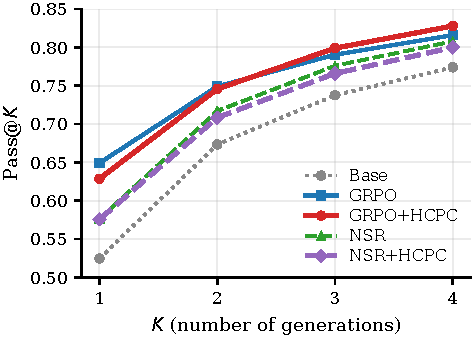
\includegraphics[width=0.95\columnwidth]{fig_passk.pdf}
\caption{Pass@$K$ on ChartQA ($n{=}500$). HCPC's gain over GRPO grows
with $K$: tied at $K{=}1$, leading at $K{=}3$ and $K{=}4$. The
direction is consistent with the design hypothesis that a
cross-rollout bonus preserves correct-path coverage at higher $K$.
Individual differences are not significant at $n{=}500$
(Pass@4 boot-$p{=}0.48$).}
\label{fig:passk}
\end{figure}

Unpacking $\Delta_{\text{tbl}}$: $P(\hat y=y^*\mid\text{tbl})$ is
$0.639$ for GRPO and $0.632$ for HCPC (tied; also tied on the
common-table intersection of 462 samples, Appendix~C), while
$P(\hat y=y^*\mid\text{no tbl})$ is $0.462$ for GRPO and $0.368$ for
HCPC. The gain therefore reflects stronger \emph{table-dependence}:
HCPC drops 9.4\,pp more than GRPO when no table is produced, while
matching it when a table is produced. The correct-path bonus makes
the extracted table load-bearing in the answer pathway.

\begin{table}[t]
\centering
\footnotesize
\setlength{\tabcolsep}{3.5pt}
\begin{tabular}{lccccc}
\toprule
Method & think & answer & type & table & order\\
\midrule
\textsc{Base}      & 52.2 & 91.2 & 96.6 & 77.2 & 81.6\\
\textsc{GRPO}      & 97.4 & 97.6 & 100  & 98.6 & 97.4\\
\textsc{GRPO+HCPC} & 98.8 & 98.2 & 100  & 99.6 & 98.6\\
\textsc{NSR}       & 57.4 & 94.8 & 96.6 & 72.2 & 85.4\\
\textsc{NSR+HCPC}  & 57.8 & 91.6 & 94.6 & 83.2 & 84.0\\
\bottomrule
\end{tabular}
\caption{Per-tag emission rate (\%) on ChartQA. Column headers refer
to the \texttt{<think>}, \texttt{<answer>}, \texttt{<type>},
\texttt{<table>} tags and the ``proper order'' check. NSR's collapse
is concentrated in the structural tags (think, table) that the base
model does not emit unprompted; HCPC under NSR partially recovers
table but not think.}
\label{tab:tags}
\end{table}

\subsection{NSR Breaks VLM Format}
\label{sec:nsr_collapse}

Switching the advantage estimator from GRPO to NSR---changing nothing
else---drops format compliance from 96.8\% to 31.6\% on ChartQA and
from 98.8\% to 16.2\% on ChartFC. The Pass@4 gap GRPO vs.\ NSR on
ChartFC is significant: $-3.8$\,pp, CI $[+0.6,+7.2]$, $p{=}0.028$
(paired bootstrap), McNemar exact $p{=}0.034$.

Table~\ref{tab:tags} localizes the collapse. NSR keeps the tags the
base model already emits ($\langle$type$\rangle$,
$\langle$answer$\rangle$, proper order) and loses the ones GRPO has to
teach ($\langle$think$\rangle$, $\langle$table$\rangle$). NSR's
$\langle$think$\rangle$ rate (57.4\%) is essentially the base model's
(52.2\%) plus noise; $\langle$table$\rangle$ rate (72.2\%) is
\emph{below} the base model's (77.2\%).

The mechanism is mechanical. Chart-RVR's structural rewards
($R_{\text{fmt}}$, $R_{\text{tok}}$, and the chart-type surrogate)
saturate quickly: emitting the required tags in the correct order is
a learned-once behavior that yields near-maximal contribution from
those components. With those rewards saturating, the total per-rollout
$R_i$ for a well-formed rollout reaches the NSR threshold
$\theta = 0.5\,R_{\max}$ regardless of whether the final answer is
correct. NSR therefore masks the advantage of
\emph{structure-good, answer-wrong} rollouts, leaving only
\emph{structure-bad, answer-wrong} rollouts---which receive negative
advantage---to drive the policy. This removes the dominant positive
gradient on structural-tag emission, and the policy drifts back toward
the base model's unstructured output. We expect this failure mode to
be absent in \citet{zhu2025nsr}'s math experiments because text-math
rewards are dominated by a single answer bit; the implicit ``format''
(a final \verb|\boxed{}| or a number on its own line) is either
trivial or emerges from the answer-correctness signal itself.
Verifying this empirically is beyond our current scope.

\subsection{HCPC Mitigates NSR's OOD Damage}
\label{sec:dissociation}

On ChartFC, HCPC added to NSR improves over plain NSR on
\emph{every metric}: Pass@1 $0.590\!\to\!0.632$ ($+4.2$\,pp),
Pass@4 $0.884\!\to\!0.894$ ($+1.0$\,pp), $\Delta_{\text{tbl}}$
$-0.059\!\to\!+0.002$ ($+0.061$), and format
$16.2\%\!\to\!17.8\%$. The $\Delta_{\text{tbl}}$ sign flip from
negative to zero indicates that table extraction stops actively
hurting; the format gain is marginal. Plain NSR is the weakest OOD
configuration in Table~\ref{tab:main} on every metric, and HCPC
closes most of that gap (Figure~\ref{fig:passk_chartfc}). How the
gap is closed (mechanism below) turns out to be more interesting
than the gap-closing itself.

\begin{figure}[t]
\centering
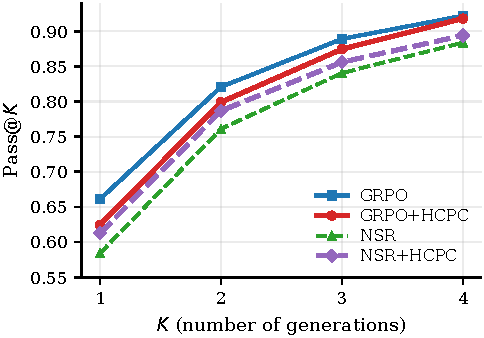
\includegraphics[width=0.95\columnwidth]{fig_passk_chartfc.pdf}
\caption{Pass@$K$ on ChartFC (OOD, $n{=}500$). Plain NSR (green)
sits below all other configurations at every $K$; adding HCPC
(purple) closes most of the gap to GRPO. \textsc{Base} was not
evaluated on ChartFC.}
\label{fig:passk_chartfc}
\end{figure}

\paragraph{Format/accuracy dissociation.} The way in which HCPC
mitigates NSR's damage is unusual: NSR+HCPC reaches Pass@1 $=0.632$,
\emph{statistically indistinguishable from GRPO} ($0.638$;
paired-bootstrap CI $[-0.046,+0.060]$, $p{=}0.85$)
\emph{while format compliance remains collapsed} at $17.8\%$ (vs.\
GRPO's $98.8\%$). In other words, HCPC under NSR recovers
GRPO-level OOD answer accuracy without recovering format. This is
the cleanest empirical evidence in the paper that format compliance
and answer accuracy are \emph{separable} downstream behaviors in
chart RLVR.

\paragraph{Why HCPC behaves so differently under GRPO and NSR.}
Under GRPO, HCPC behaves as designed: the bonus is added to
correct-path rollouts' rewards, those rollouts get higher GRPO
advantage $(R_i - \bar R)/s_R$, and the policy is reinforced toward
the correct path. This is the standard positive-gradient
interpretation and accounts for the ChartQA results
(\S\ref{sec:hcpc_grpo}).

Under NSR, the same bonus operates through a different channel.
HCPC adds its bonus to exactly the correct-path rollouts that NSR
then masks out of the gradient---so the bonus does not reach the
policy as a direct positive update. But TRL computes the GRPO
advantage \emph{before} the NSR mask is applied, using the group
mean $\bar R$ over the full set of rollouts. Adding $B_{\text{HCPC}}$
to correct rollouts raises $\bar R$, and for the wrong rollouts that
survive the mask this makes their advantage more negative. The
correct-path bonus therefore reshapes the reference baseline that
the surviving (wrong) rollouts are penalized against, pushing the
policy harder away from wrong-path behavior. The mechanism is
\emph{baseline shift, not direct reinforcement}: HCPC under NSR
strengthens the negative gradient on wrong rollouts without
providing any positive gradient on correct ones. This is consistent
with what we observe---answer-level OOD accuracy recovers because
wrong-rollout suppression strengthens, while structured-output
emission (which requires positive gradient on correct rollouts that
neither NSR nor HCPC-under-NSR can provide) remains collapsed.

On ChartQA, adding HCPC on top of NSR also partially restores format
($31.6\%\!\to\!43.0\%$ overall, with the recovery concentrated in
$\langle$table$\rangle$: $72.2\%\!\to\!83.2\%$, Table~\ref{tab:tags}).
The asymmetry between ID and OOD---partial format recovery on ID,
near-zero format recovery on OOD despite full accuracy recovery on
OOD---is what makes the channel-separability claim concrete.

\section{Related Work}

\paragraph{Chart-reasoning training.} Chart-RVR \citep{chartrvr2025}
is the closest baseline---a verifiable-reward GRPO pipeline for chart
QA with surrogate rewards on chart type and table reconstruction. We
use its rewards verbatim as $R_{\text{base}}$ and add cross-rollout
signal; our deltas isolate the effect of the group-level term against
the same per-rollout backbone. Other recent chart VLMs improve
training data \citep{chartgemma,chartinstruct,bigcharts2025},
reasoning rationales \citep{chartr12025,chartqax2026,distill-vcr-2025},
or wrap models in agentic pipelines
\citep{chartagent2025,vprochart2025,chartcitor2025,chartpoint2025};
these are complementary to our reward-side intervention. Benchmarks
beyond ChartQA include ChartX/ChartVLM \citep{chartx2024} and the
style-OOD sets EvoChart \citep{evochart} and ChartQAPro
\citep{chartqapro}; we leave style-OOD evaluation as future work.

\paragraph{RLVR and its decomposition.} \citet{zhu2025nsr} are the
only prior work to isolate positive- vs.\ negative-sample
reinforcement; we test their recipe in a multi-component multimodal
reward landscape and document the format-collapse failure mode that
does not appear in their text-only math setting.
\citet{su2025crossing,wen2025rlvr,rlvmr2025,koksal2025fewshot}
study RLVR in other settings but do not address the
multi-component-reward asymmetry we identify.

\paragraph{Self-consistency and group-level signals.} \citet{wang2022sc}
aggregate by majority vote at inference; \citet{ettrl2025} balance
exploration and exploitation at test time. HCPC differs in being a
training-time, group-level reward that conditions on ground-truth
correctness rather than majority agreement, and that targets
level-specific objectives (consistent extraction, diverse reasoning)
rather than a single aggregate.

\section{Conclusion}

We introduced HCPC, a cross-rollout bonus that preserves
correct-path diversity in chart RLVR by conditioning on ground-truth
correctness and rewarding consistent extraction together with diverse
reasoning. On Qwen2.5-VL-3B, GRPO+HCPC matches the Chart-RVR baseline
on Pass@1 and produces consistently more robust correct groups
($40.8\%$ all-4-correct vs.\ $38.6\%$; Pass@4 $0.828$ vs.\ $0.816$;
$\Delta_{\text{tbl}}$ $+0.264$ vs.\ $+0.178$). Comparing against
Negative-Sample Reinforcement, an alternative diversity-preservation
recipe imported from text-only math RLVR, we find that NSR ported
unchanged collapses format compliance in chart RLVR ($96.8\%$ to
$31.6\%$) and significantly hurts OOD Pass@4, because structural
rewards saturate quickly enough for well-formed rollouts to cross
NSR's correctness threshold regardless of answer quality. Adding HCPC
on top of NSR recovers GRPO-level OOD accuracy at near-zero format
compliance via a baseline-shift mechanism in the GRPO advantage,
empirical evidence that format and answer accuracy are separable
behavioral channels of the trained policy. The takeaway for
practitioners: advantage-rule asymmetries developed for single-reward
source domains can interact destructively with reward components the
source domain did not have, and the shape of the multi-component
reward mixture deserves to be a first-class consideration when
porting RLVR recipes across modalities.

\section*{Limitations}

We use a single 3B-parameter backbone (Qwen2.5-VL-3B), a 1{,}000-sample
training subset, $K{=}4$ rollouts, and a 500-sample test slice per
benchmark. Compute constraints prevented us from training on the full
Chart-RVR CoT mixture (34{,}194 samples), evaluating on the full
ChartQA and ChartFC test sets, or running EvoChart \citep{evochart}
and ChartQAPro \citep{chartqapro} as style-OOD benchmarks distinct
from the joint task-and-style probe ChartFC provides. Scaling to the
full training data, full test sets, and a style-only OOD benchmark is
our highest-priority follow-up.

Headline accuracy differences between HCPC and GRPO are within
paired-bootstrap noise; HCPC's positive evidence is in
$\Delta_{\text{tbl}}$ and in the dissociation under NSR rather than
in raw accuracy. HCPC's $D_{\text{reason}}$ component is small in
absolute terms because reasoning traces for the same chart question
are near-duplicates in MiniLM space at $K{=}4$; we report it as part
of the reward but do not claim it as a primary metric. Two NSR fixes
suggested by \S\ref{sec:nsr_collapse} (component-aware advantages,
threshold calibration) are not evaluated.

% Custom bibliography entries only
\bibliography{custom}

\appendix

\section{Reproducibility}
\label{sec:appendix}

All training and evaluation code, model checkpoints, and per-sample
evaluation outputs (for the 500-sample test slices of ChartQA and
ChartFC) are released with the paper. Training uses 4 generations per
prompt at training temperature 1.0; evaluation uses 4 generations at
temperature 0.8 and top-$p{=}0.95$. Pass@$K$ uses the unbiased
estimator of \citet{passatk}. Cross-rollout similarities use
MiniLM-L6 embeddings. Paired-bootstrap CIs use
$n_{\text{boot}}{=}10{,}000$ resamples; McNemar tests use the
two-sided exact binomial form on the discordant pair.

\section{Qualitative Example: Format Collapse in Action}
\label{sec:qualitative}

Figure-free illustration of the NSR collapse and HCPC partial
recovery, on a single ChartQA sample where the question is
\emph{``How many categories are there in the chart?''} with ground
truth $y^* = $ \texttt{4}. We show rollout 0 from three methods.

\paragraph{GRPO (correct, well-formed).}
\begin{quote}\footnotesize\ttfamily
<{}think><{}type>pie</type><{}table>\{\dots,~"rows":~[["Asians","63"],\dots]\}</table>
<{}step-1> The chart is a pie chart\dots
<{}step-4> Based on the information provided, there are four distinct categories\dots
</think>
<{}answer>4</answer>
\end{quote}

\paragraph{NSR (format-collapsed; arrives at right reasoning but
wrong answer surface form).}
\begin{quote}\footnotesize\ttfamily
<{}think>First, I'll identify the type of chart and the underlying
data table\dots
<{}step-1> The chart shows four categories: Asians, Whites, Blacks,
and Hispanics. \dots
Final answer:\\
Four\\
</think>
<{}answer>Four</answer>
\end{quote}
NSR's rollout contains no \texttt{<table>} tag, no \texttt{<type>}
tag, and emits the reasoning steps inline rather than as structured
items. The answer is also expressed in word form (``Four'') rather
than the numeric form the eval expects (``4''), so the strict-match
metric marks it incorrect despite the reasoning being substantively
right.

\paragraph{NSR+HCPC (table tag recovered; answer still in word
form).}
\begin{quote}\footnotesize\ttfamily
<{}think><{}type>bar</type><{}table>\{"columns":~["Country","Bar~Color"],"rows":~[["Asians","\dots"],\dots]\}</table>
<{}step-1>From the chart\dots
<{}step-3>\dots there are four distinct categories.
</think>
<{}answer>Four</answer>
\end{quote}
HCPC's group-level bonus on $C_{\text{table}}$ pulls NSR's policy
back toward emitting a \texttt{<table>} tag (table fraction
$72.2\%\!\to\!83.2\%$ on ChartQA, Table~\ref{tab:tags}). The chart
type is incorrectly identified (\texttt{bar} instead of \texttt{pie}),
illustrating that HCPC's partial format recovery is not the same as a
full quality recovery---and the answer is still ``Four'' in word
form. This is exactly the dissociation pattern of
\S\ref{sec:dissociation}: format is partly restored, but the
answer-surface alignment that drives strict-match accuracy is
governed by a separate channel.

\section{Per-Answer-Type Breakdown}

We split ChartQA test samples by ground-truth answer type. Pass@1
differences between \textsc{GRPO} and \textsc{GRPO+HCPC} are within
exact-McNemar noise on numeric ($n{=}302$, $-1.7$\,pp, $p{=}0.63$),
boolean ($n{=}75$, $+4.0$\,pp, $p{=}0.71$), and string ($n{=}114$,
$-6.1$\,pp, $p{=}0.30$). HCPC does not provide a category-specific
accuracy advantage at this scale.

\section{$\Delta_{\text{tbl}}$ on the Common-Table Subset}

To rule out the confound that $\Delta_{\text{tbl}}$ is computed on
different denominators per method, we recompute it on the
intersection of samples where multiple methods produce a parseable
table. On the 462 ChartQA samples where both \textsc{GRPO} and
\textsc{GRPO+HCPC} produce parseable tables,
$P(\hat y=y^*\mid\text{tbl})$ is 0.643 vs.\ 0.636. The
$\Delta_{\text{tbl}}$ gap in Table~\ref{tab:main} therefore arises
entirely from the $P(\hat y=y^*\mid\text{no tbl})$ arm
(0.462 vs.\ 0.368). We interpret this as evidence that HCPC induces
stronger \emph{table-dependence}, not stronger table-conditioned
reasoning accuracy.

\end{document}
